\documentclass{ctexart}
\usepackage{tikz}
\begin{document}
textwidth=\the\textwidth

linewidth=\the\linewidth

hsize=\the\hsize

paperwidth=\the\paperwidth

parindent=\the\parindent

leftskip=\the\leftskip

rightskip=\the\rightskip

columnwidth=\the\columnwidth


When we have to specify a length depending on current conditions, we have to use the correct parameter. 

\begin{tikzpicture}[remember picture,overlay]
\draw[red,thick](0,0) rectangle (\textwidth,-.8);
\draw[red](.3\textwidth,-.8)--(.3\textwidth,.2) node {30\%};
\end{tikzpicture}


	\begin{minipage}[c][1.5em][c]{.3\textwidth}
	30\%,\the\textwidth
	\end{minipage}
	\begin{minipage}[c][1.5em][c]{.7\textwidth}
	70\%, \the\textwidth,\the\linewidth
	\end{minipage}
	
\begin{enumerate}
	\item
	\the\textwidth,\the\linewidth
	\begin{enumerate}
\item
\the\textwidth,\the\linewidth
\end{enumerate}
\end{enumerate}

全球聚焦北京,“一带一路”国际合作高峰论坛举行,{\the\textwidth}多国政要云集北京,看中国长袖善舞......

\end{document}